% =================================================================================================
% File:			pianificazione.tex
% Description:	Defiinisce la sezione relativa alla pianificazione delle attività nelle diverse fasi del ciclo di vita
% Created:		2014-12-30
% Author:		Tesser Paolo
% Email:		tesser.paolo@mashup-unipd.it
% =================================================================================================
% Modification History:
% Version		Modifier Date		Change											Author
% 0.0.1 		2014-12-30 			creata struttura base pianificazione			Tesser Paolo
% =================================================================================================
% 0.0.2			2015-01-02			Definizione periodi fasi e inizio stesura		Tesser Paolo
% =================================================================================================
% 0.0.3			2015-01-07			continuata stesura sulle attività da svolgere	Tesser Paolo
% =================================================================================================
%

% CONTENUTO DEL CAPITOLO

\section{Pianificazione} % (fold)
\label{sec:pianificazione}
I diagrammi delle attività presenti in questa sezione sono stati rappresentati tramite l'uso dei diagrammi di Gantt.
	\subsection{Ricerca e implementazione degli strumenti} % (fold)
	\label{sub:ricerca_e_implementazione_degli_strumenti}
	\textbf{Periodo}: 2014-11-26 - 2014-12-08 \\
	Questa fase comincia con la presentazione delle regole e delle scadenze da parte del committente e termina con un giorno scelto dal \roleProjectManager{} nel quale le scelte principali sugli strumenti e la loro implementazione sono state ritenute sufficienti per proseguire alla fase seguente. \\
	Le attività che verranno svolte sono:
		\begin{itemize}
			\item \textbf{Ricerca degli strumenti}: l'\roleAdministrator{} ha il compito di scegliere i principali strumenti che servono per il lavoro collaborativo. In particolare quelli per redigere la documentazione, il sistema di ticketing e il repository. Dovrà inoltre trovare/creare degli script che automatizzino i controlli per conformare il lavoro svolto con le \docNameVersionNdP;
			\item \textbf{Apprendimento degli strumenti}: tutti i membri del gruppo dovranno documentarsi sugli strumenti scelti per apprenderne il funzionamento, qualora non conoscessero già come utilizzarli, grazie anche ai documenti informativi condivisi dall'\roleAdministrator;
			\item \textbf{Implementazione degli strumenti}: l'\roleAdministrator{} avrà il compito di implementare e configurare gli strumenti trovati.
		\end{itemize}
	\noindent
	Nonostante la terminazione di questa fase sia fissata in un giorno preciso, la ricerca di strumenti più efficienti e migliorativi per l'avanzamento del progetto deve essere sempre portata avanti da parte dell'\roleAdministrator.
	 	
		\subsubsection{Diagramma delle attività} % (fold)
		\label{ssub:diagramma_delle_attivita}
			\begin{figure}[htbp]
				% \centering
				\centerline{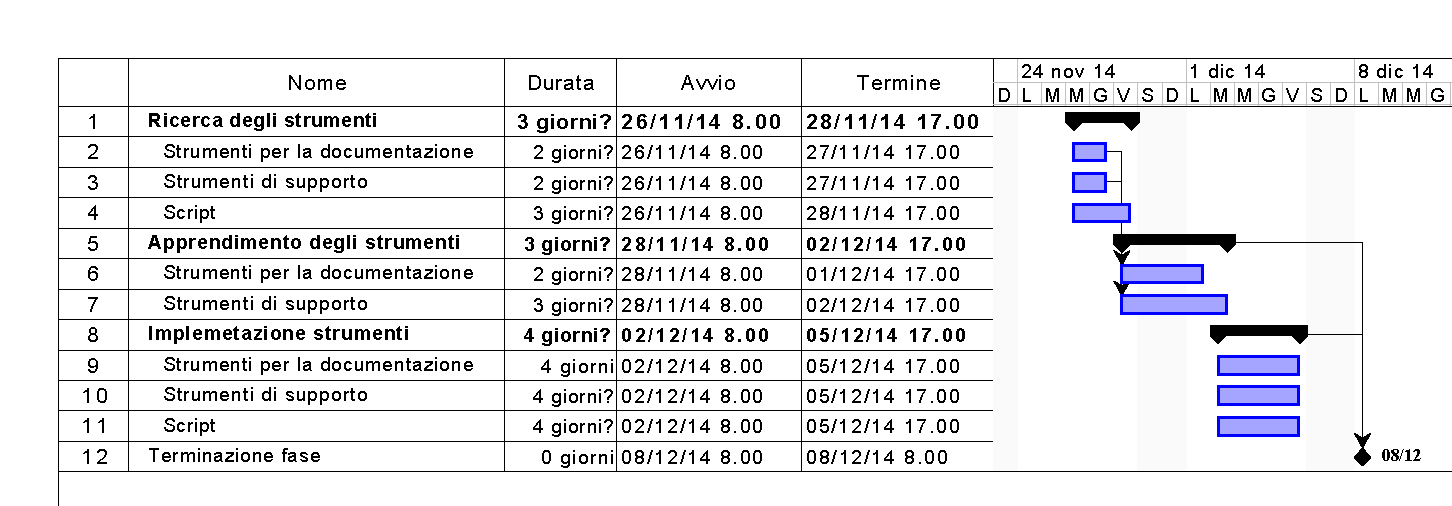
\includegraphics[scale=0.7]{images/d_attivita_fase_implem_strumenti.pdf}}
				\caption{Diagramma di Gantt - Ricerca e implementazione degli strumenti}
				\label{fig:gantt_ricerca_e_implementazione_strumenti}				
			\end{figure}
		% subsubsection diagramma_delle_attività (end)
	% subsection ricerca_e_implementazione_degli_strumenti (end)
	
	\subsection{Analisi dei requisiti} % (fold)
	\label{sub:analisi_dei_requisiti}
	\textbf{Periodo}: 2014-12-08 - 2015-01-22 \\
	Questa fase comincia dopo la scelta e l'implementazione degli strumenti necessari a definire il repository utilizzato dal team e le strutture di base per redigere la documentazione. Terminerà con la scadenza di consegna dell'offerta, cioè con la consegna della \RR. \\
	Le attività che verranno svolte sono:
		\begin{itemize}
			\item \textbf{Norme di Progetto}: l'\roleAdministrator{} una volta implementati gli strumenti di scrittura dei documenti, potrà iniziare a redarre le \docNameVersionNdP;
			\item \textbf{Studio di Fattibilità}: gli \emph{Analisti} devono valutare tutti i capitolati proposti e redarre lo \docNameVersionSdF{} al termine del quale si andrà a decidere il capitolo;
			\item \textbf{Analisi dei Requisiti}: gli \emph{Analisti} iniziano la ricerca dei requisiti e la loro stesura nel documento \docNameVersionAdR{}. Questa attività comprende anche degli incontri con il proponente;
			\item \textbf{Piano di Progetto}: il \roleProjectManager{} andrà a pianificare le attività che i membri del gruppo andranno a svolgere. Le decisioni prese andranno documentate nel \docNameVersionPdP;
			\item \textbf{Piano di Qualifica}: i \emph{Verificatori} dovranno redigere il \docNameVersionPdQ;
			\item \textbf{Glossario}: viene redatto il \docNameVersionGlo;
			\item \textbf{Incontri}: verranno effettuati degli incontri con il proponente per analizzare i requisiti fino a quel momento trovati e avere un riscontro se si sta procedendo nella direzione corretta o meno.
		\end{itemize}
	
		\subsubsection{Diagramma delle attività} % (fold)
		\label{ssub:diagramma_delle_attivita}
			\begin{figure}[htbp]
				\centering
				\centerline{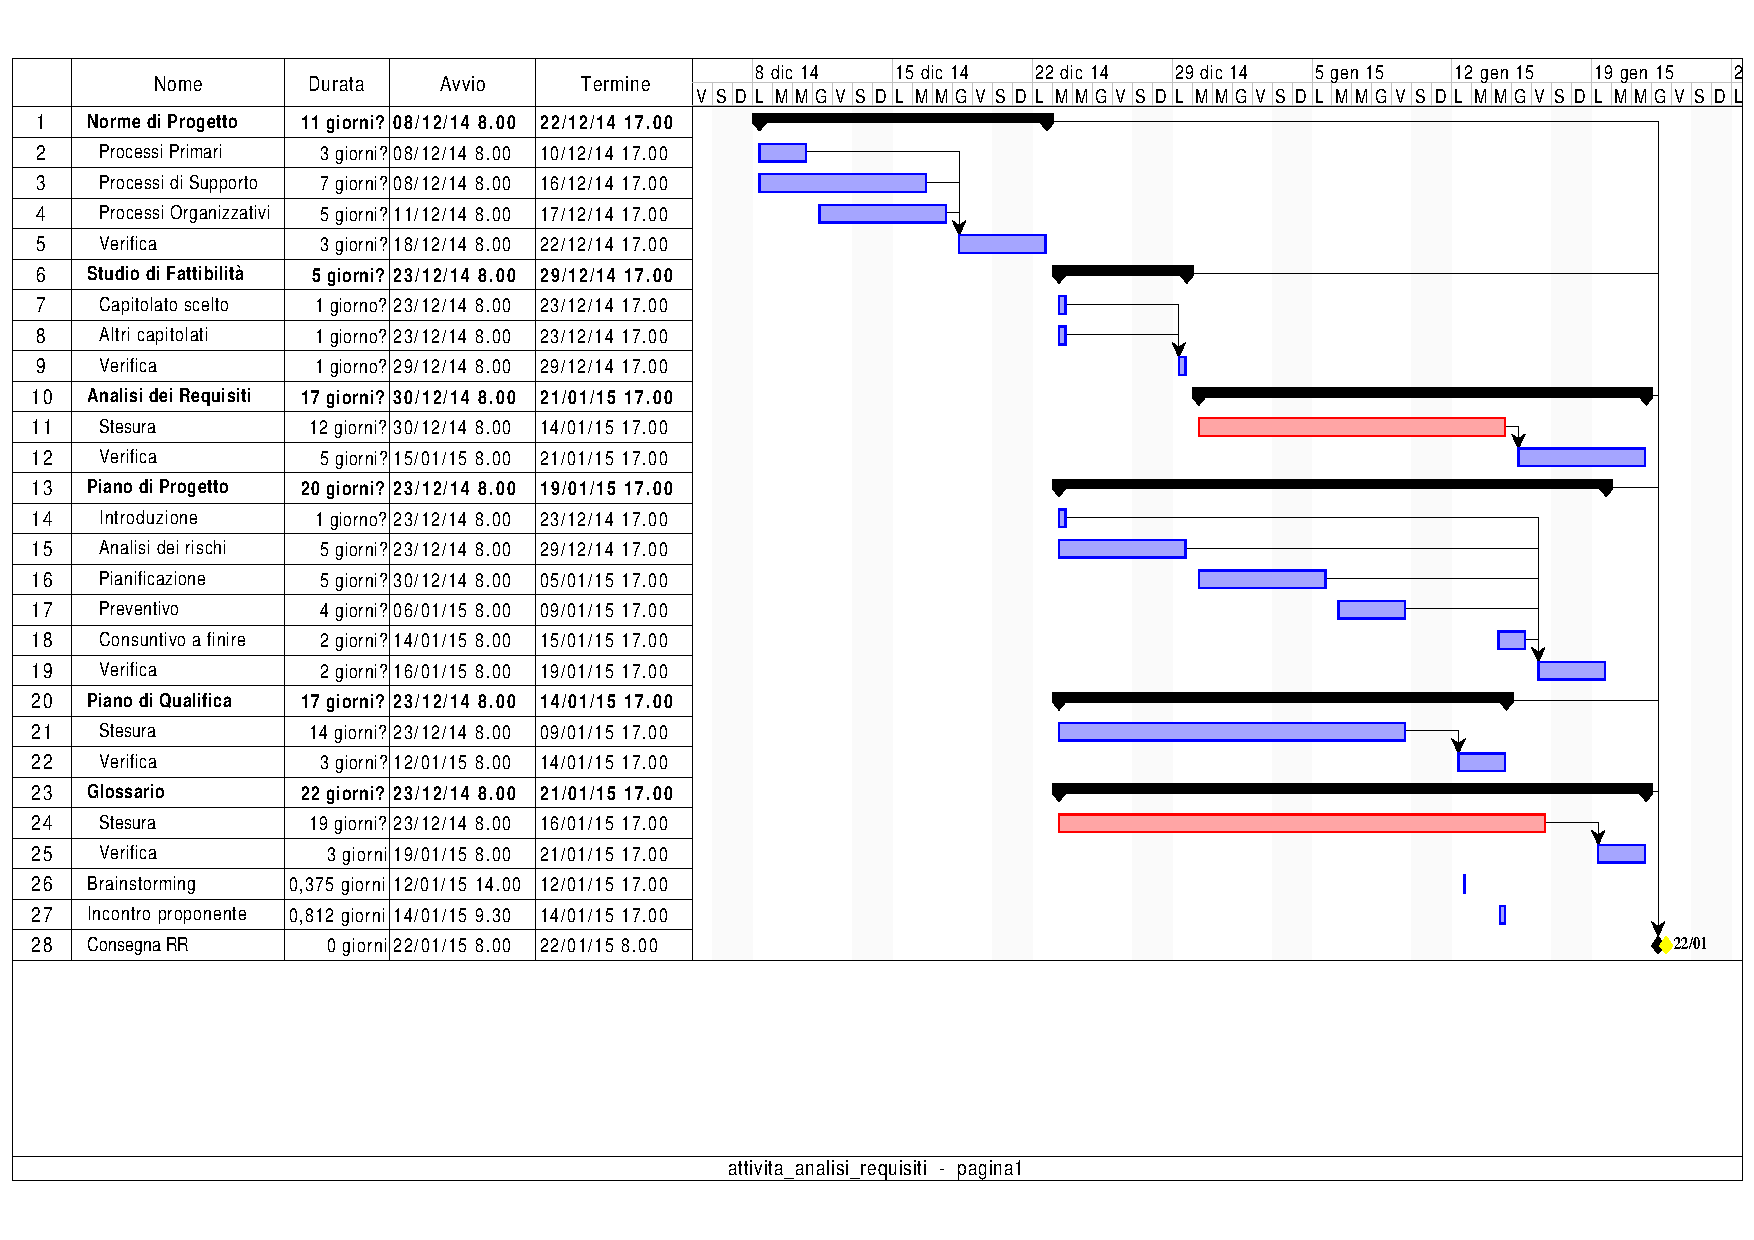
\includegraphics[scale=0.7]{images/d_attivita_analisi_requisiti.pdf}}
				\caption{Diagramma di Gantt - Analisi dei requisiti}
				\label{fig:gantt_analisi_requisiti}				
			\end{figure}
		% subsubsection diagramma_delle_attività (end)
	% subsection analisi_dei_requisiti (end)
	
	
	\subsection{Analisi di dettaglio} % (fold)
	\label{sub:analisi_di_dettaglio}
	\textbf{Periodo}: 2015-01-27 - 2015-02-16 \\
	Questa fase comincia qualche giorno dopo il termine della consegna della \RR{} e termina con la \RR{} stessa.
	Le attività che verranno svolte sono:
		\begin{itemize}
			\item \textbf{Analisi di dettaglio}: gli \emph{Analisti} andranno a consolidare i requisiti trovati e a migliorare il documento di \docNameVersionAdR;
			\item \textbf{Incremento e Verifica}: i documenti già redatti verranno aggiornati e migliorati;
			\item \textbf{Preparazione della presentazione}: vengono svolte delle attività per prepararsi ad affrontare la presentazione della \RR.
		\end{itemize}
	
		\subsubsection{Diagramma delle attività} % (fold)
		\label{ssub:diagramma_delle_attivita}
			\begin{figure}[htbp]
				\centering
				\centerline{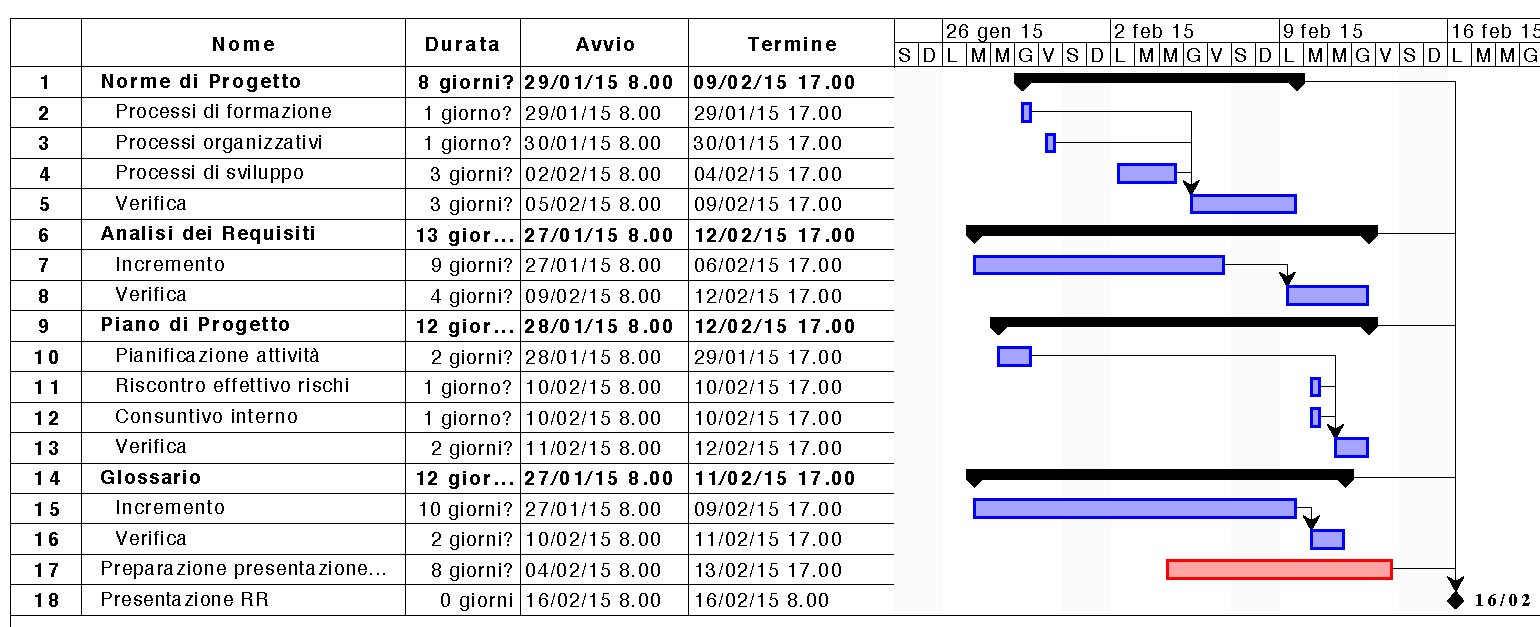
\includegraphics[scale=0.7]{images/d_attivita_analisi_dettaglio.pdf}}
				\caption{Diagramma di Gantt - Analisi di dettaglio}
				\label{fig:gantt_analisi_dettaglio}				
			\end{figure}
		% subsubsection diagramma_delle_attività (end)
	% subsection analisi_di_dettaglio (end)
	
	\subsection{Progettazione architetturale} % (fold)
	\label{sub:progettazione_architetturale}
	\textbf{Periodo}:  2015-02-17 - 2015-03-23 \\
	Questa fase comincia un giorno dopo della \RR{} e termina con un incontro con il proponente.
	Le attività che verranno svolte sono:
		\begin{itemize}
			\item \textbf{Specifica Tecnica}: il \roleDesigner{} ha il compito di fornire delle scelte progettuali di alto livello del prodotto finale. Il tutto verrà redatto nel documento \docNameVersionST{} che conterrà i design pattern che verranno utilizzati e l'architettura a grandi linee del prodotto;
			\item \textbf{Incremento e Verifica}: i documenti già redatti verranno aggiornati e migliorati a seconda del risultato ottenuto nella \RR;
			\item \textbf{Incontro con il proponente}: viene effettuato un incontro con il proponente per valutare se le scelte fatte sono conformi alle aspettative.
		\end{itemize}
		
		\subsubsection{Diagramma delle attività} % (fold)
		\label{ssub:diagramma_delle_attivita}
			\begin{figure}[htbp]
				\centering
				\centerline{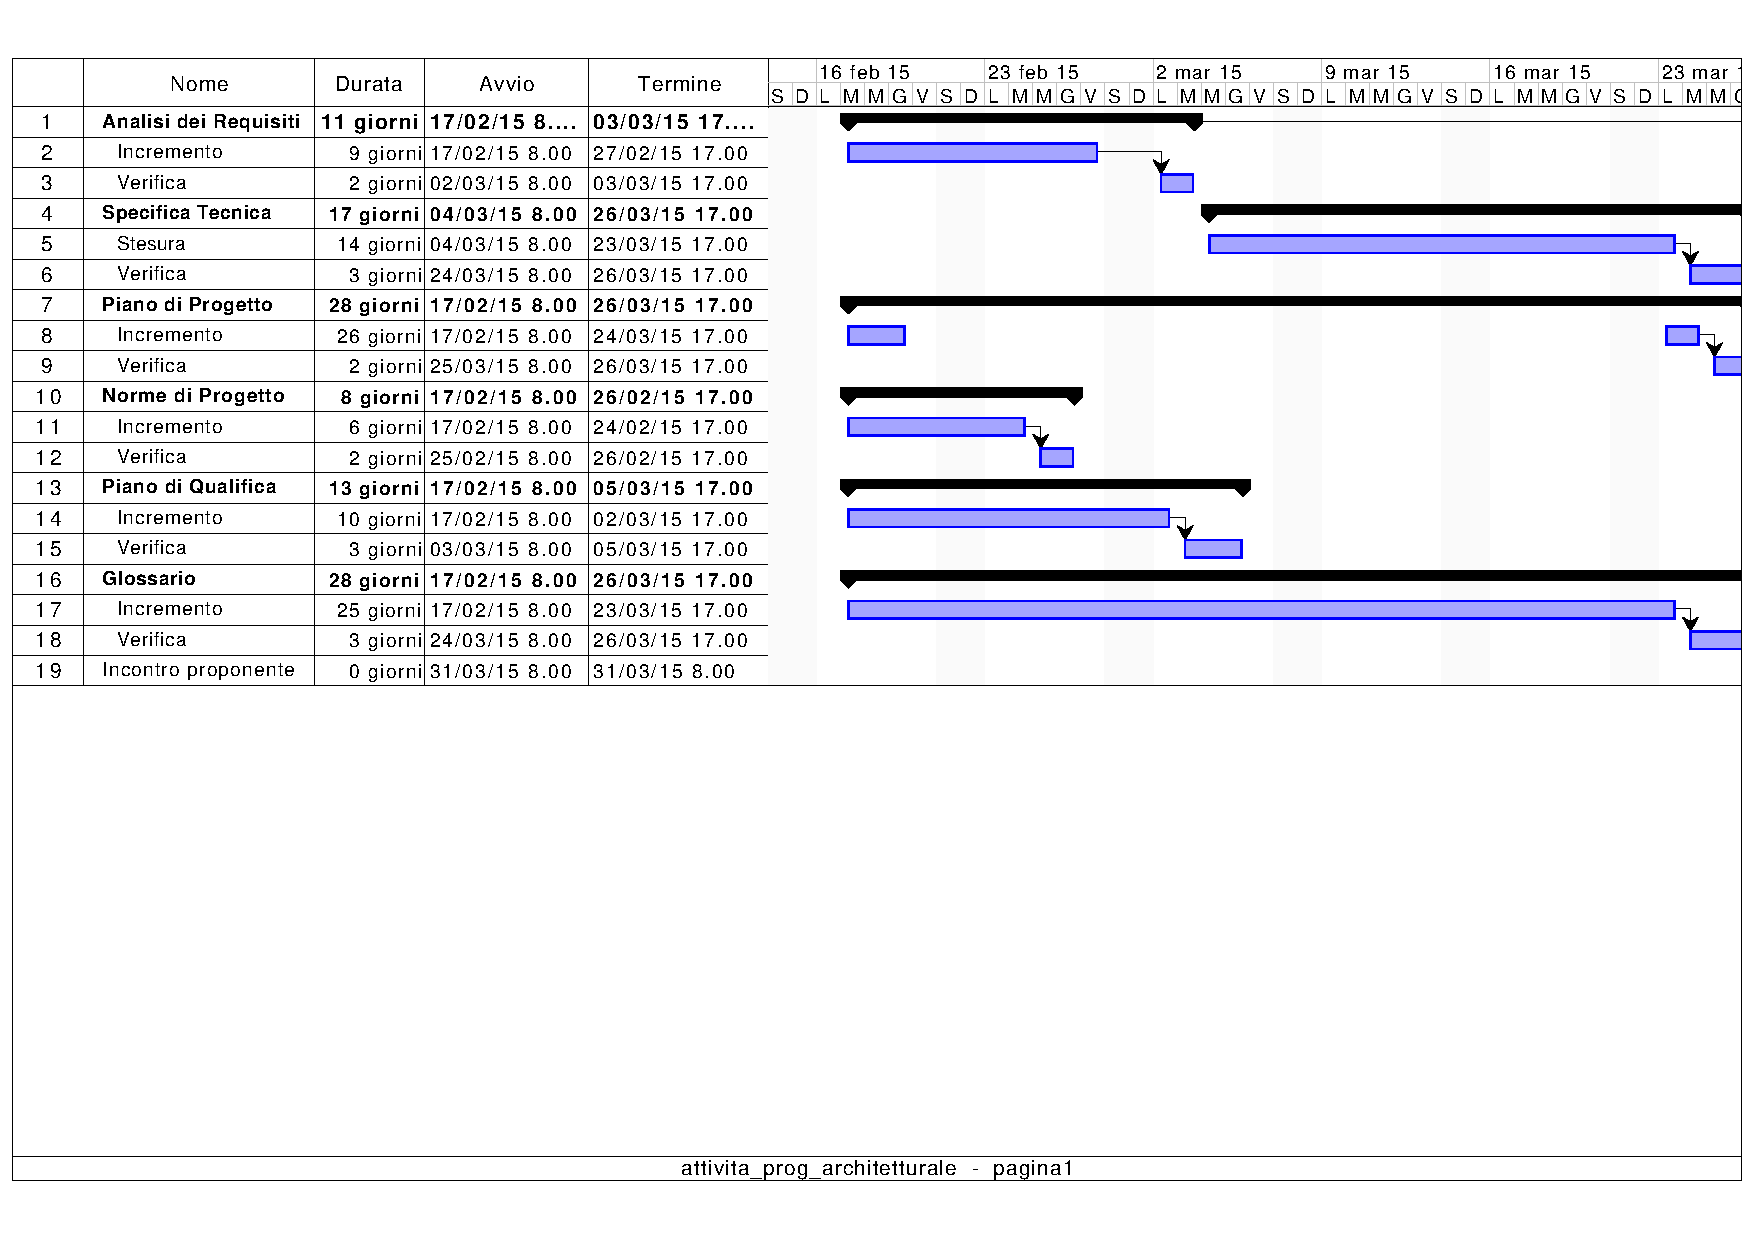
\includegraphics[scale=0.7]{images/d_attivita_prog_architetturale.pdf}}
				\caption{Diagramma di Gantt - Progettazione architetturale}
				\label{fig:gantt_prog_architetturale}				
			\end{figure}
		% subsubsection diagramma_delle_attività (end)
	% subsection progettazione_architetturale (end)
	
	\subsection{Progettazione di dettaglio e codifica dei requisiti obbligatori} % (fold)
	\label{sub:progettazione_di_dettaglio_e_codifica_dei_requisiti_obbligatori}
	\textbf{Periodo}:  2015-03-24 - 2015-04-27 \\
	Questa fase comincia dopo l'incontro con il proponente per avere delle valutazioni sulla fase di progettazione architetturale svolta e termina con la presentazione del lavoro svolto in fase di \RPmin;
	Le attività che verranno svolte sono:
		\begin{itemize}
			\item \textbf{Definizione di Prodotto}: viene redatta la \docNameDdP{} \emph{v1.0.0} relativa alla parte inerente ai requisiti obbligatori. In esso verranno definiti con profondità la struttura e le relazioni dei vari componenti del sistema basandosi sulla \docNameVersionST;
			\item \textbf{Manuale utente}: viene iniziata la redazione del \docNameVersionMU{} che servirà per fornire indicazione agli utilizzatori del sistema;
			\item \textbf{Codifica}: i \emph{Programmatori} iniziano lo sviluppo del codice del prodotto necessario al soddisfacimento dei requisiti obbligatori. Per la codifica andrà seguito il documento di \docNameVersionDdP;
			\item \textbf{Incremento e Verifica}: i documenti già redatti verranno aggiornati e migliorati a seconda del riscontro ottenuto dall'incontro con il proponente;
			\item \textbf{Preparazione della presentazione}: vengono svolte delle attività per prepararsi ad affrontare la presentazione della \RPmin;
			\item \textbf{Consegna}: andranno consegnati al committente i documenti relativi alla fase di progettazione architetturale esposta nella sezione \ref{sub:progettazione_architetturale}. La consegna andrà effettuata in data 2015-04-20;
			\item \textbf{Incontro con il proponente}: viene effettuato un incontro con il proponente per ricevere un feedback sul lavoro svolto per soddisfare i requisiti obbligatori trovati. \\
			L'incontro sarà fissato nella settimana che va dal 2015-04-20 al 2015-04-24;
		\end{itemize}
		
		\subsubsection{Diagramma delle attività} % (fold)
		\label{ssub:diagramma_delle_attivita}
			\begin{figure}[htbp]
				\centering
				\centerline{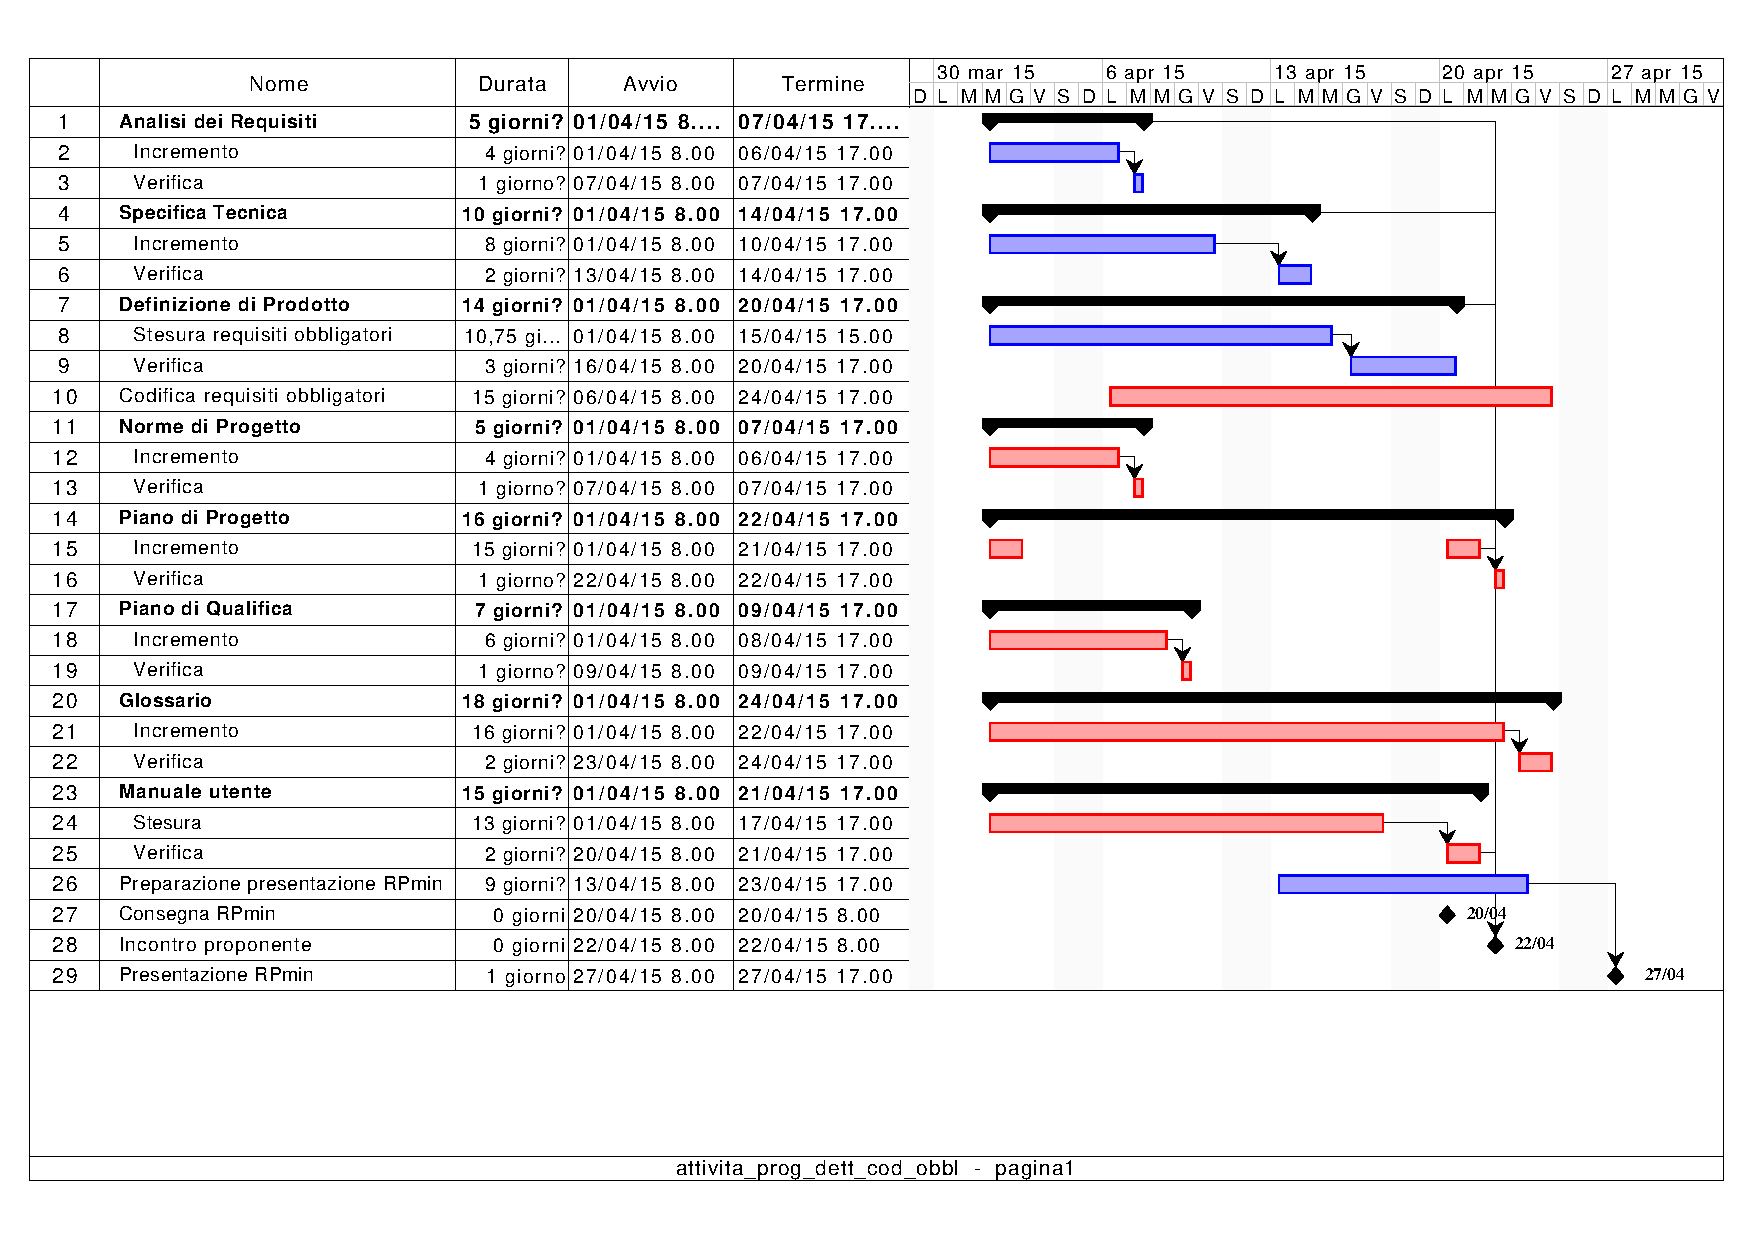
\includegraphics[scale=0.7]{images/d_attivita_prog_dett_cod_obbl.pdf}}
				\caption{Diagramma di Gantt - Progettazione di dettaglio e codifica dei requisiti obbligatori}
				\label{fig:gantt_prog_dett_cod_requisiti_obbligatori}				
			\end{figure}
		% subsubsection diagramma_delle_attività (end)
	% subsection progettazione_di_dettaglio_e_codifica_dei_requisiti_obbligatori (end)
	
	\subsection{Progettazione di dettaglio e codifica dei requisiti desiderabili} % (fold)
	\label{sub:progettazione_di_dettaglio_e_codifica_dei_requisiti_desiderabili}
	\textbf{Periodo}:  2015-04-28 - 2015-05-11 \\
	Questa fase comincia dopo la \RPmin{} e termina con un altro incontro con il proponente per ricevere un feedback sul lavoro svolto per soddisfare i requisiti desiderabili trovati.
	Le attività che verranno svolte sono:
		\begin{itemize}
			\item \textbf{Definizione di Prodotto}: viene redatta la \docNameVersionDdP{} relativa alla parte inerente ai requisiti desiderabili. In esso verranno definiti con profondità la struttura e le relazioni dei vari componenti del sistema basandosi sulla \docNameVersionST;
			\item \textbf{Codifica}: i \emph{Programmatori} iniziano lo sviluppo del codice del prodotto necessario al soddisfacimento dei requisiti desiderabili. Per la codifica andrà seguito il documento di \docNameVersionDdP;
			\item \textbf{Incremento e Verifica}: i documenti già redatti verranno aggiornati e migliorati a seconda del riscontro ottenuto dall'incontro con il proponente e dall'esito della \RPmin.
		\end{itemize}
		
		\subsubsection{Diagramma delle attività} % (fold)
		\label{ssub:diagramma_delle_attivita}
			\begin{figure}[htbp]
				\centering
				\centerline{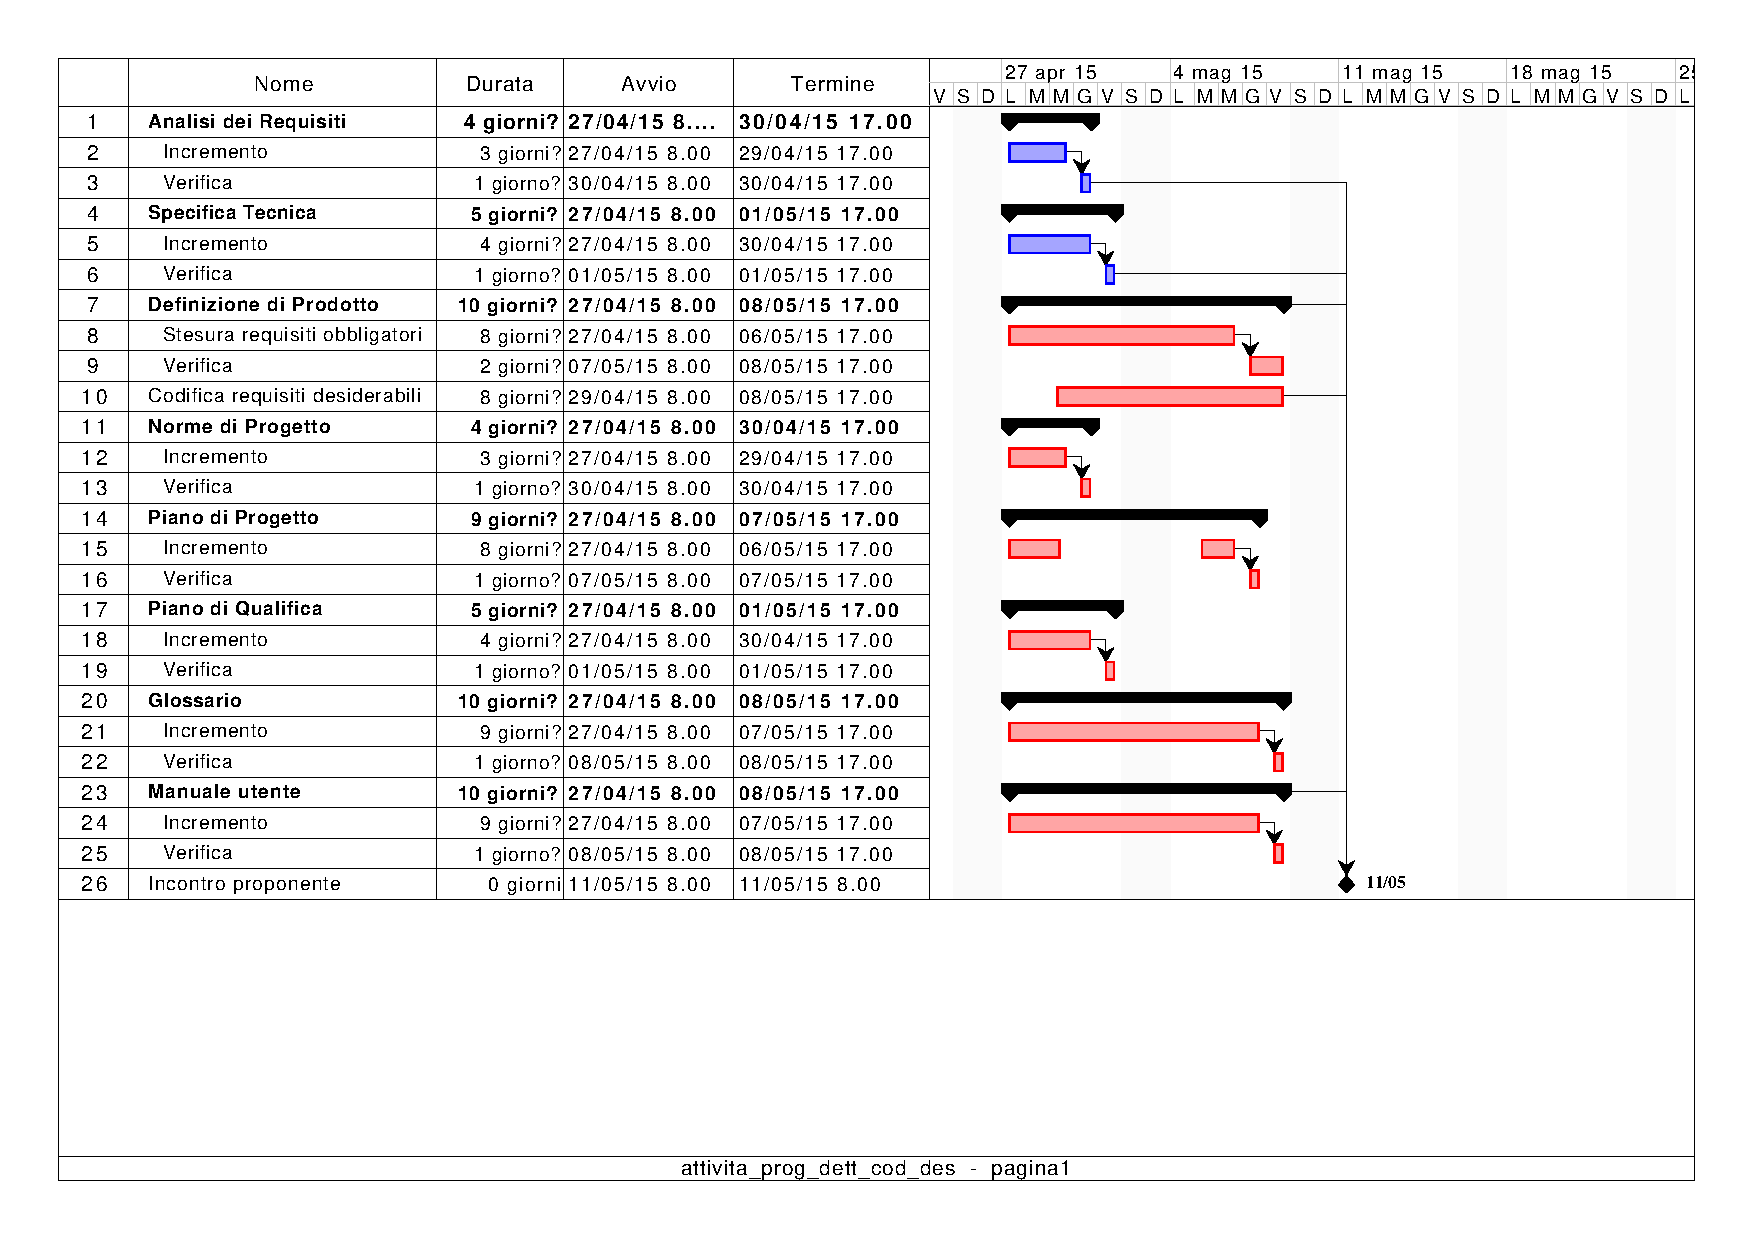
\includegraphics[scale=0.7]{images/d_attivita_prog_dett_cod_des.pdf}}
				\caption{Diagramma di Gantt - Progettazione di dettaglio e codifica dei requisiti desiderabili}
				\label{fig:gantt_prog_dett_cod_requisiti_desiderabili}				
			\end{figure}
		% subsubsection diagramma_delle_attività (end)
	% subsection progettazione_di_dettaglio_e_codifica_dei_requisiti_desiderabili (end)
	
	\subsection{Progettazione di dettaglio e codifica dei requisiti opzionali} % (fold)
	\label{sub:progettazione_di_dettaglio_e_codifica_dei_requisiti_opzionali}
	\textbf{Periodo}:  2015-05-12 - 2015-05-21 \\
	Questa fase comincia dopo l'incontro con il proponente per la valutazione sui requisiti desiderabili e termina con la consegna della \RQ.
	Le attività che verranno svolte sono:
		\begin{itemize}
			\item \textbf{Definizione di Prodotto}: viene redatta la \docNameVersionDdP{} relativa alla parte inerente ai requisiti opzionali. In esso verranno definiti con profondità la struttura e le relazioni dei vari componenti del sistema basandosi sulla \docNameVersionST;
			\item \textbf{Codifica}: i \emph{Programmatori} iniziano lo sviluppo del codice del prodotto necessario al soddisfacimento dei requisiti opzionali. Per la codifica andrà seguito il documento di \docNameVersionDdP;
			\item \textbf{Incremento e Verifica}: i documenti già redatti verranno aggiornati e migliorati a seconda del riscontro ottenuto dall'incontro con il proponente;
			\item \textbf{Preparazione della presentazione}: vengono iniziate le attività per prepararsi ad affrontare la presentazione della \RQ{} che continueranno nella fase seguente.
		\end{itemize}
			
		\subsubsection{Diagramma delle attività} % (fold)
		\label{ssub:diagramma_delle_attivita}
			\begin{figure}[htbp]
				\centering
				\centerline{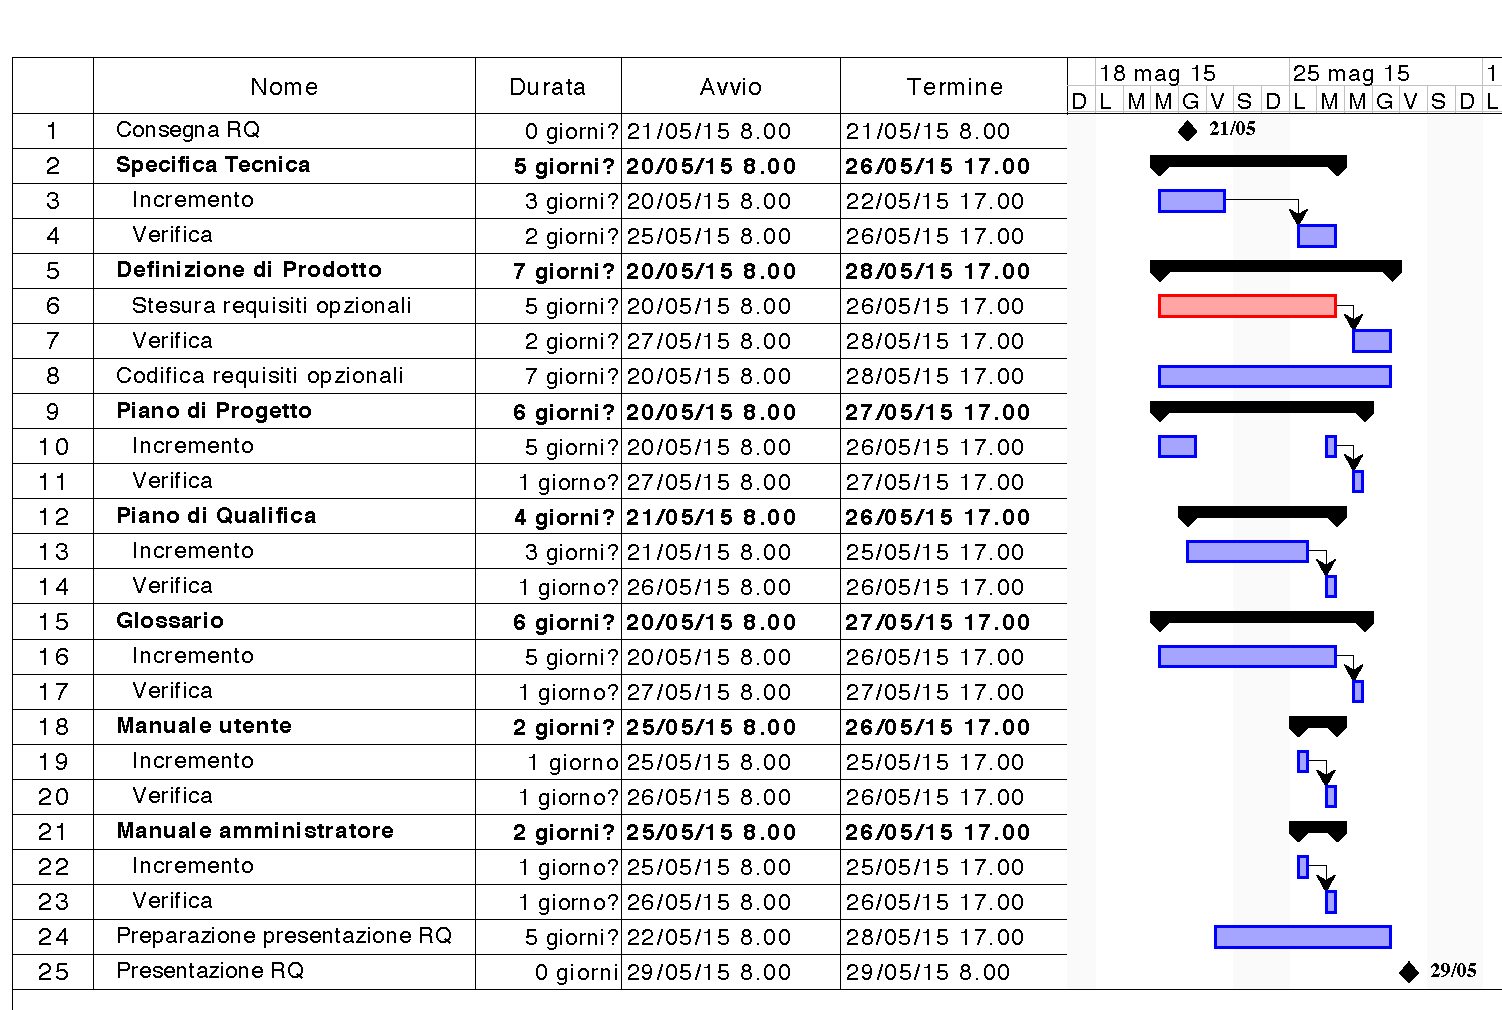
\includegraphics[scale=0.7]{images/d_attivita_prog_dett_cod_opz.pdf}}
				\caption{Diagramma di Gantt - Progettazione di dettaglio e codifica dei requisiti opzionali}
				\label{fig:gantt_prog_dett_cod_requisiti_opzionali}				
			\end{figure}
		% subsubsection diagramma_delle_attività (end)
	% subsection progettazione_di_dettaglio_e_codifica_dei_requisiti_opzionali (end)
	
	\subsection{Validazione} % (fold)
	\label{sub:validazione}
	\textbf{Periodo}:  2015-05-22 - 2015-06-17 \\
	Questa fase comincia dopo la consegna della \RQ{} e termina con la consegna della \RA.
	Le attività che verranno svolte sono:
		\begin{itemize}
			\item \textbf{Preparazione della presentazione - RQ}: vengono terminate le attività per prepararsi ad affrontare la presentazione della \RQ;
			\item \textbf{Presentazione \RQ}: viene effettuata la presentazione relativa alla consegna effettuata in data 2015-05-21 della \RQ;
			\item \textbf{Incremento e Verifica}: i documenti già redatti verranno aggiornati e migliorati a seconda dall'esito della \RQ;
			\item \textbf{Validazione e collaudo}: il prodotto viene eseguito e testato per dimostrare che è conforme alle specifiche e soddisfa i requisiti proposti al proponente;
			\item \textbf{Preparazione della presentazione - RA}: vengono svolte delle attività per prepararsi ad affrontare la presentazione della \RA;
		\end{itemize}
		
		\subsubsection{Diagramma delle attività} % (fold)
		\label{ssub:diagramma_delle_attivita}
			\begin{figure}[htbp]
				\centering
				\centerline{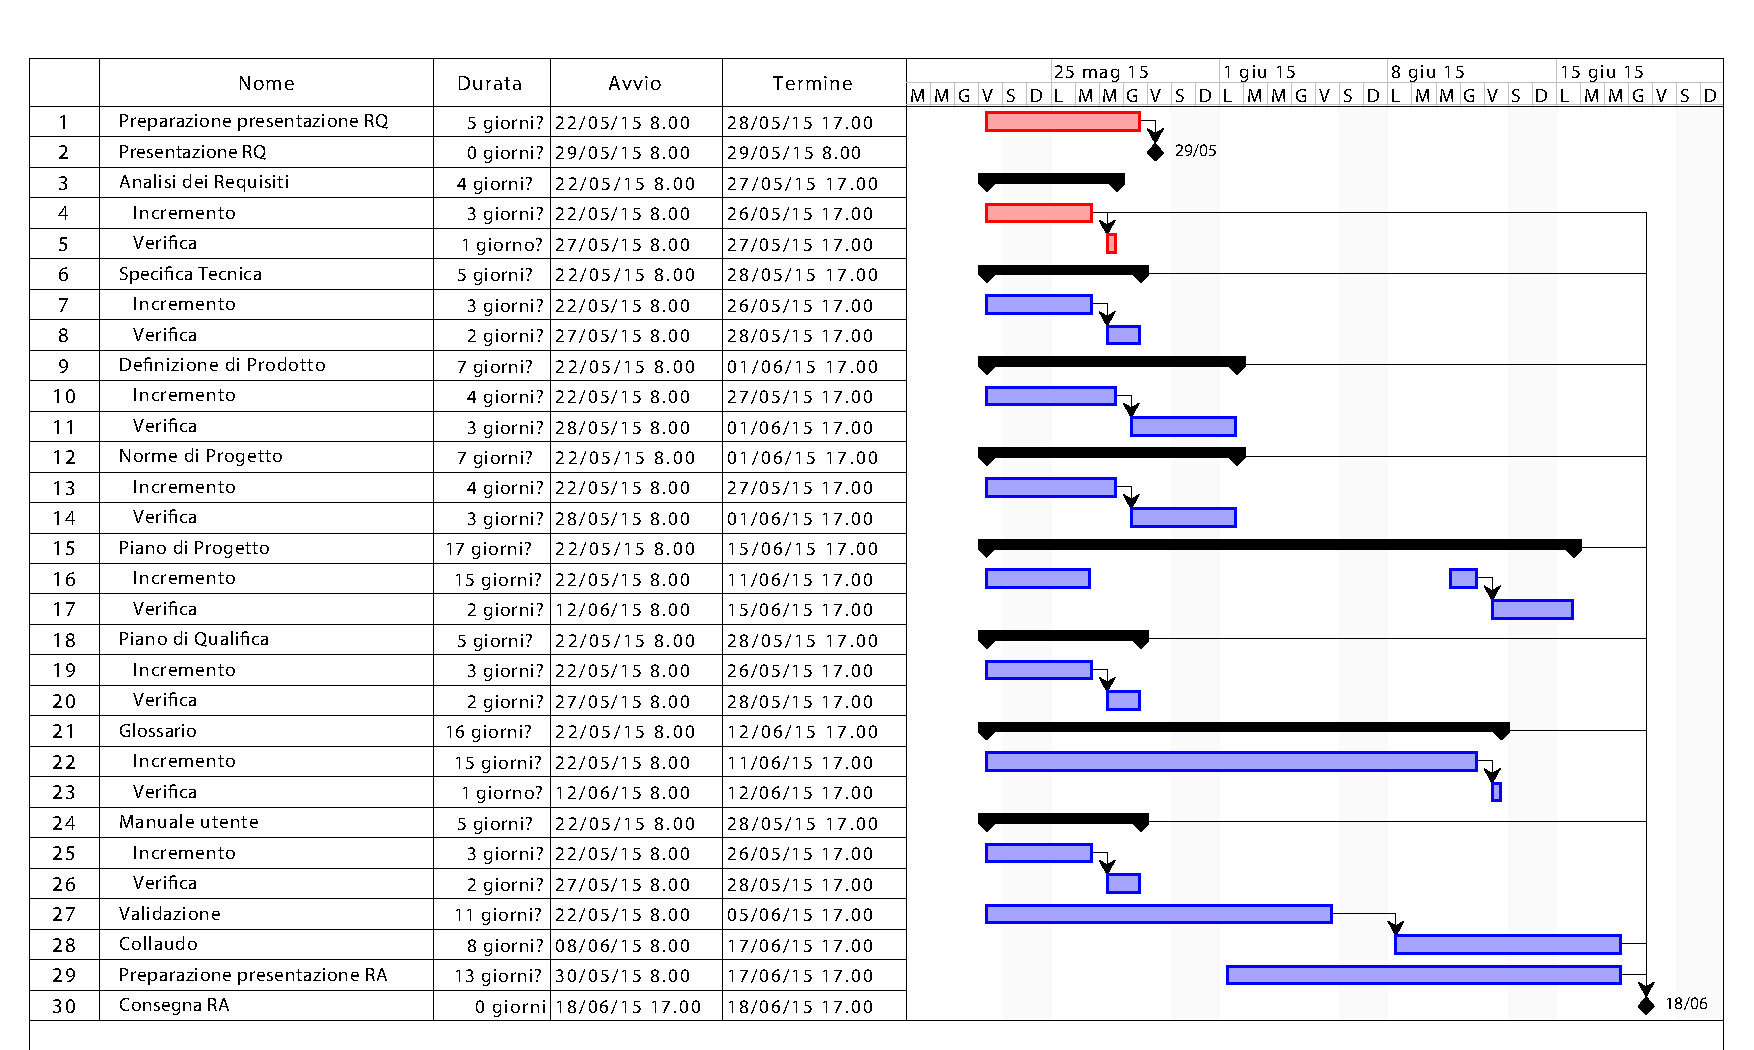
\includegraphics[scale=0.7]{images/d_attivita_validazione.pdf}}
				\caption{Diagramma di Gantt - Validazione}
				\label{fig:gantt_validazione}				
			\end{figure}
		% subsubsection diagramma_delle_attività (end)
	% subsection validazione (end)
	
	
% section pianificazione (end)